\documentclass[10pt]{article}
\usepackage[margin=1in]{geometry}
\usepackage{times}
\usepackage[T1]{fontenc}
\usepackage{microtype}
\usepackage{amsmath,amssymb}
\usepackage{booktabs}
\usepackage{graphicx}
\usepackage[numbers,sort&compress]{natbib}
\usepackage{xcolor}
\usepackage[colorlinks=true,linkcolor=blue!50!black,citecolor=blue!50!black,urlcolor=blue!50!black]{hyperref}
\usepackage{caption}
\captionsetup{font=small}
\makeatletter\newcommand{\tabinput}[1]{\@@input #1 }\makeatother

\title{Is There a ``Sounds Like AI'' Direction in the Residual Stream?\\[2pt]
\large Reading, Writing and Disentangling Chat-Assistant Style in Qwen2.5-7B}
\author{Anonymous authors}
\date{}

\begin{document}
\maketitle

\begin{abstract}
Human-written and AI-written text are known to be linearly separable in LLM activations. We ask whether the separating direction is also \emph{causal} for generation, and whether it is anything more than a relabelling of formality, fluency, domain, length or the Assistant persona. In Qwen2.5-7B-Instruct we fit a diff-of-means ``AI direction'' on question-matched and prefix-matched human/AI pairs, cut to equal token length. It transfers to unseen generators (GPT-4, GPT-4o, Llama-3-Instruct) and to content-matched paraphrases, but not to base-model or pre-chat LM text, so it encodes \emph{chat-assistant} style rather than machine authorship. About half of its norm lies in the span of six authorship-controlled confound directions. Projecting that span out makes it a \emph{better} read-out (AUROC 0.97--0.99). Subtracting the direction at one layer while the model answers held-out questions moves two supervised detectors from P(AI)$=$0.99 to 0.33--0.42, and moves the zero-shot Binoculars score to the level of real human answers. Among answers an LLM judge rates highly coherent and relevant, the confound-orthogonal direction reaches P(AI) 0.40/0.30, matching real human answers (0.36/0.26). Equal-norm random, formality, fluency and register directions leave detection at 0.95--1.00, the Assistant axis reaches only 0.72, and a ``write like a human'' prompt leaves 99\% of answers flagged. Adding the direction yields stock assistant prose, including in the base model. The direction is nearly identical in the pretrained base model (cosine $\geq$0.98 at every layer), so chat tuning did not create it. We also report failure modes (language switching, coherence loss at high strength, brittle multi-layer ablation) and find that an LLM judge cannot tell human from AI text in our setting.
\end{abstract}

\section{Introduction}
\label{sec:intro}

Large language models (LLMs) encode many high-level properties of text along approximately linear directions of the residual stream: truthfulness~\citep{marks2024geometry,li2023inference}, refusal~\citep{arditi2024refusal}, sentiment and style~\citep{turner2023steering,konen2024style}, persona traits~\citep{chen2025persona}, and the default ``Assistant'' persona itself~\citep{lu2026assistant}. Adding or removing such a direction during generation often changes the corresponding property of the model's output~\citep{zou2023representation,rimsky2024steering}. A natural question is whether \emph{sounding like an AI} is another such property.

The read-out half of that question is mostly settled. Human-written and machine-written text are linearly separable in LLM activations: linear probes beat many dedicated detectors and recover a shared machine-text direction~\citep{quaremba2026linear}, per-layer human-vs-AI steering vectors work as detectors~\citep{vishnyakov2026svdetect}, and sparse-autoencoder features of Gemma-2-2B separate the two~\citep{kuznetsov2025feature}. All of this work is about \emph{detection}. Two questions remain open. First, is the direction \emph{causal for generation}? If we add or subtract it while the model writes, does its output read as more or less AI-written to an \emph{independent} detector, with content and coherence preserved? Second, what \emph{is} the direction? Human and AI corpora differ in formality, fluency (perplexity), domain, length and verbosity, and AI text is written in the voice of the Assistant persona. A separating direction could just be one of these, relabelled.

We study both questions in Qwen2.5-7B-Instruct and its pretrained base model, using matched corpora, explicit confound directions, and a steering protocol with equal-norm controls. Our contributions:
\begin{enumerate}
    \item \textbf{Read-out, with length and content control.} A diff-of-means ``AI direction'' fit on question-matched (HC3) and prefix-matched (human-AI parallel corpus) pairs, with every pair cut to the same token length, transfers to held-out generators (GPT-4o, Llama-3-Instruct, GPT-4 on MAGE) and to content-matched paraphrases. It does \emph{not} detect text from base (non-chat) LMs or older pre-chat generators (AUROC $\approx$0.5--0.65). So it encodes chat-model style, not machine authorship as such.
    \item \textbf{Disentanglement.} The raw direction is about half confound: $\sim$54\% of its squared norm at layer 12 lies in the span of six confound directions (formality, register, domain, fluency, verbosity, Assistant axis), and it has cosine 0.6--0.7 with formality and fluency but only 0.3--0.4 with the Assistant axis. Projecting that span out does \emph{not} remove the signal. The remaining confound-orthogonal component $u_{AI}^{\perp}$ is a \emph{better} detector (AUROC 0.97--0.99 vs.\ 0.83--0.86 on matched sets at layer 12).
    \item \textbf{Causality.} Subtracting the direction at one middle layer makes the instruct model's answers read as human to two independent supervised detectors and a zero-shot detector (Binoculars): P(AI) falls from 0.99 to 0.33--0.42, close to real human answers. An LLM judge we planned as a third measure turned out unable to tell human from AI text, so we use it only for coherence. Matched-norm random directions do nothing, and confound directions do less. We characterise the coherence cost and compare with a ``write like a human'' prompt at matched coherence (\S\ref{sec:steer}).
    \item \textbf{Base vs.\ instruct.} The direction is already present in the pretrained base model. Base and instruct directions have cosine $\geq 0.98$ at every layer, with equal read-out AUROC, so chat tuning did not create or amplify it. Adding the direction to the base model makes its continuations of human text read as AI-written.
\end{enumerate}

\section{Related work}
\label{sec:related}

\paragraph{Machine-generated text detection.} Detectors split into supervised classifiers, trained on human and machine text from benchmarks such as HC3~\citep{guo2023hc3}, MAGE~\citep{li2024mage} and RAID~\citep{dugan2024raid}, and zero-shot statistics such as DetectGPT~\citep{mitchell2023detectgpt} and Binoculars~\citep{hans2024binoculars}. Paraphrasing can evade detectors, and reliable detection may be impossible in principle~\citep{krishna2023paraphrasing,sadasivan2023can}. Closest to us, \citet{quaremba2026linear} show that linear probes on LLM activations are strong and robust detectors that recover a shared machine-text direction. \citet{vishnyakov2026svdetect} use per-layer human-vs-AI steering vectors \emph{as detectors}. \citet{kuznetsov2025feature} interpret Gemma-2-2B SAE features~\citep{lieberum2024gemmascope} for detection and steer some features to interpret them. None of these asks whether the read-out direction controls how AI-like the model's own writing reads to an independent detector, or what the direction is beyond a detector.

\paragraph{Stylistic signatures of LLM text.} LLM text overuses particular words~\citep{kobak2025delving,liang2024monitoring,liang2024mapping}, differs from human text in grammatical and rhetorical features even when continuing the same prefix~\citep{reinhart2025llms}, and carries model-specific idiosyncrasies~\citep{sun2025idiosyncrasies}. We use the parallel corpus of \citet{reinhart2025llms} as a prefix-matched contrast.

\paragraph{Linear representations and steering.} Under the linear representation hypothesis~\citep{park2024linear}, many concepts are directions that can be read with probes and written with activation additions~\citep{turner2023steering,zou2023representation,li2023inference,rimsky2024steering}. Some are mediated by a single direction~\citep{arditi2024refusal}. Style vectors steer output style~\citep{konen2024style}, and persona vectors steer character traits~\citep{chen2025persona}. \citet{lu2026assistant} find a dominant ``Assistant axis'' for the default persona that already exists in base models. We test whether the AI-text direction is that axis. To remove confounds we use linear subspace erasure, as in INLP and LEACE~\citep{ravfogel2020null,belrose2023leace}.

\section{Setup}
\label{sec:method}

\paragraph{Models and representations.} We study Qwen2.5-7B-Instruct and its pretrained base Qwen2.5-7B~\citep{qwen2025qwen25} (28 layers, $d{=}3584$). $h_\ell$ denotes the residual stream after block $\ell$. To \emph{read} a text we feed it as raw text (no chat template). We cut it to at most 128 tokens and mean-pool $h_\ell$ over all positions except the first, which is an attention sink with outlier norm. \textbf{Length control:} the members of a matched group (the human and AI answers to one question, or the human and model continuations of one prefix) are cut to the \emph{same} number of tokens, the minimum over the group. Pooled representations therefore never see a length difference within a pair.

\paragraph{Corpora.} Table~\ref{tab:data} summarises the data. \textbf{HC3}~\citep{guo2023hc3}: one human and one ChatGPT answer per question, in five domains (Reddit ELI5 is capped so it does not dominate). HC3 human answers carry Penn-Treebank tokenisation artefacts (``do n't'', `` .''), which would be a trivial cue. We detokenise \emph{both} sides with the same rules. \textbf{HAP}, the human-AI parallel corpus~\citep{reinhart2025llms}: for 1{,}800 documents in six genres (academic, blog, fiction, news, spoken, TV/movie) we pair the true human continuation of a prefix with the continuations of GPT-4o, GPT-4o-mini, Llama-3-8B/70B-Instruct and Llama-3-8B/70B \emph{base}~\citep{grattafiori2024llama3}. \textbf{MAGE}~\citep{li2024mage} is used for out-of-distribution evaluation only. It has 1{,}200 human texts, 600 from chat-style generators (GPT-3.5-turbo, text-davinci-003), 600 from older LMs (OPT, FLAN-T5, T0, LLaMA-1, GLM, BLOOM, GPT-J/NeoX), and its GPT-4 OOD set. \textbf{Rewrites}: 500 human training passages rewritten by Llama-3.1-8B-Instruct, a different model family, in a formal, an informal and a neutral-paraphrase version. HC3 and HAP are split 70/30 by question or document. All directions are fit on training splits only. A further 160 HC3 questions (40 each from ELI5, open QA, finance and medicine) are held out entirely as steering prompts.

\begin{table}[t]
\centering\small
\caption{Data. ``Matched'' = groups share a question or a prefix and are length-matched in tokens.}
\label{tab:data}
\begin{tabular}{llrl}
\toprule
Corpus & Contrast & Texts & Use\\
\midrule
HC3 & human vs ChatGPT, same question & 6{,}230 & fit $u_{AI}$ (train) / eval (test), matched\\
HAP & human vs 6 LMs, same prefix & 12{,}600 & fit $u_{AI}$ (instruct LMs, train) / eval, matched\\
MAGE & human vs 30+ generators, 10 domains & 2{,}400 & OOD eval\\
MAGE-GPT4 & human vs GPT-4 & 1{,}562 & OOD eval\\
Rewrites & human / formal / informal / paraphrase & 2{,}000 & formality direction; content-matched eval\\
Persona responses & default Assistant vs 24 role-play personas & 400 & Assistant axis\\
\bottomrule
\end{tabular}
\end{table}

\paragraph{Directions.} All directions are differences of means, unit-normalised per layer. The \textbf{AI direction} is $u_{AI} = \mathrm{unit}(\hat u_{HC3} + \hat u_{HAP})$, where $\hat u_{HC3}$ is the ChatGPT-minus-human direction on HC3 and $\hat u_{HAP}$ is the instruct-LM-minus-human direction on HAP (GPT-4o, GPT-4o-mini, Llama-3-Instruct). Pooling two corpora with different topics and generators averages out corpus-specific confounds. Six \textbf{confound directions} each hold \emph{authorship fixed}:
\textit{formality} (formal minus informal Llama rewrite of the same passage, both AI);
\textit{register} (HAP human academic+news minus spoken+TV+fiction, both human);
\textit{domain} (HC3 human encyclopedic domains minus Reddit ELI5);
\textit{fluency} (human texts in the lowest minus the highest tertile of per-token NLL under the model);
\textit{verbosity} (HC3 human answers in the longest minus the shortest tertile of full length);
and the \textit{Assistant axis}, after \citet{lu2026assistant}: the model answers 16 questions as its default Assistant and in 24 role-play personas (pirate, nurse, detective, \dots). We mean-pool the residual stream over response tokens inside the chat template and take default minus role-play. Finally, $u_{AI}^{\perp}$ is $u_{AI}$ with the span of the six confound directions projected out, renormalised.

\paragraph{Read-out evaluation.} We report the AUROC of the scalar projection $h_\ell^\top u$ on held-out sets. A logistic-regression probe on all $d$ dimensions (standardised, $C{=}0.01$), trained on the same data, gives an upper bound. For the \emph{nullspace test} we project the confound span out of all activations, refit the diff-of-means on the training data, and re-evaluate. We compare against removing a random subspace of the same dimension, and against removing $u_{AI}$ itself.

\paragraph{Steering.} Following activation addition~\citep{turner2023steering}, we add $\alpha\, g_\ell\, v$ to $h_\ell$ at every position (prompt and generated) at a single layer $\ell$. Here $v$ is a unit direction and $g_\ell$ is the human-to-AI gap: the difference between the mean AI and mean human projections on $u_{AI}$ in the training data ($g_{12}{=}7.1$). So $\alpha{=}{-}1$ moves the activations by one human-to-AI gap towards human. A pilot over layers $\{8,12,16,20,24\}$ on 40 prompts (Appendix~\ref{app:pilot}) picked $\ell{=}12$, which gave the largest detector change per unit of coherence loss. We sweep $\alpha\in\{\pm2,\pm4,\pm6,\pm8\}$.
\textbf{Controls} use \emph{exactly the same vector norm}: three isotropic random directions; the formality, register, fluency and Assistant directions; and $u_{AI}^{\perp}$.
\textbf{Prompt baseline}: a system prompt asking the model to answer like an ordinary person on a forum such as Reddit, ``not like an AI assistant''. We also combine this prompt with negative steering.
\textbf{Multi-layer variants}: adding $\alpha\, g_\ell\, u_{AI,\ell}$ at all layers 1--27 with $\alpha\in\{\pm0.25,\pm0.5,\pm1\}$, and clamping every token's projection on $u_{AI,\ell}$ to the human (or AI) mean at all layers (a directional ablation).
Every condition answers the same 160 held-out HC3 questions with the chat template (temperature 0.7, top-$p$ 0.9, at most 200 new tokens), using the same random seed across conditions. A second unsteered run with a different seed measures sampling variability.

\paragraph{Independent measures.} No measure has access to Qwen activations.
(i)~Two public supervised detectors: \texttt{desklib/ai-text-detector-v1.01} (DeBERTa-v3-large trained on recent LLM text) and \texttt{fakespot-ai/roberta-base-ai-text-detection-v1}. A third, the HC3-trained \texttt{Hello-SimpleAI/chatgpt-detector-roberta}, is reported only for completeness: it was trained on the corpus we fit $u_{AI}$ on.
(ii)~The zero-shot Binoculars score~\citep{hans2024binoculars} with Falcon-7B and Falcon-7B-Instruct~\citep{almazrouei2023falcon}. We report $-B$, so that higher means more AI-like.
(iii)~An LLM judge, Gemma-3-12B-it~\citep{gemma2025gemma3}, a different model family, run at temperature 0~\citep{zheng2023judging}. It rates each response 1--10 for \emph{AI-likeness}, \emph{coherence} and \emph{relevance} to the question.
For fluency we use the mean token NLL under Falcon-7B. For content preservation we use the cosine similarity between all-mpnet-base-v2 embeddings~\citep{reimers2019sentence,song2020mpnet} of each steered answer and the unsteered answer to the same question. We also compute simple stylometrics: length, list items, first-person rate, contractions, and the rate of stock ``AI phrases''. We validate every measure on held-out \emph{real} human and AI text (Table~\ref{tab:validation}).

\section{Results}
\label{sec:results}

\subsection{Read-out: a chat-model-text direction that transfers, but not to base or older LMs}
\label{sec:readout}

\begin{table}[t]
\centering\small
\caption{Held-out AUROC of read-out directions (Qwen2.5-7B-Instruct). $u_{AI}$ and $u_{AI}^{\perp}$ are projections onto one direction, at layer 12 (L12; the steering layer) and layer 27. ``Probe'' is a full-dimensional logistic probe trained on the same data (L12). ``$-$NLL'' uses only the text's mean token log-likelihood under the model. ``Best conf.'' is the best single confound direction (formality, register, fluency, domain or Assistant axis). The last three columns are the nullspace test at L12: refit diff-of-means after removing the 6-dim confound span, a random 6-dim subspace, or $u_{AI}$ itself. $^\dagger$Same corpus family as training (test split).}
\label{tab:readout}
\setlength{\tabcolsep}{3.5pt}
\begin{tabular}{lccccccccc}
\toprule
& \multicolumn{3}{c}{direction} & & & & \multicolumn{3}{c}{refit after removing \dots}\\
\cmidrule(lr){2-4}\cmidrule(lr){8-10}
Eval set & $u_{AI}$ L12 & $u_{AI}^{\perp}$ L12 & $u_{AI}$ L27 & Probe & $-$NLL & Best conf. & confounds & random & $u_{AI}$\\
\midrule
\tabinput{tables/readout.tex}
\bottomrule
\end{tabular}
\end{table}

\begin{figure}[t]
\centering
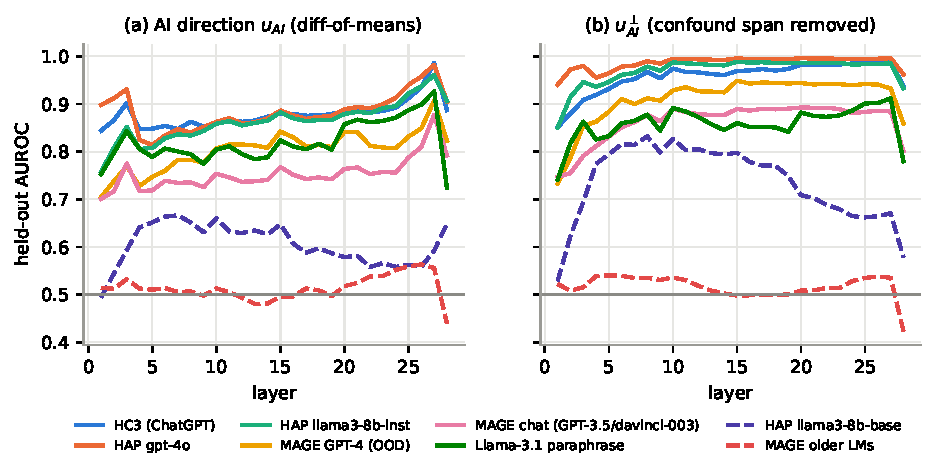
\includegraphics[width=\linewidth]{figures/readout_layers.pdf}
\caption{Held-out AUROC across layers (instruct model). Dashed lines are machine text \emph{not} from chat-tuned models (Llama-3 base continuations, pre-2022 LMs); the direction does not detect it.}
\label{fig:readout_layers}
\end{figure}

Table~\ref{tab:readout} and Figure~\ref{fig:readout_layers} reproduce the read-out result of prior work under stricter controls. A single diff-of-means direction, fit on length-matched pairs, separates held-out human and chat-model text at every layer. AUROC is 0.83--0.86 in the middle layers and up to 0.98 at layer 27. The full probe reaches 0.93--1.00. The direction transfers to generators and corpora never used for fitting: GPT-4 on MAGE (0.81 at L12, 0.91 at L27) and GPT-3.5/davinci-003 (0.74/0.88). It also transfers to Llama-3.1 \emph{paraphrases} of the very human passages they are compared with (0.79/0.93). There, topic, content and length are held fixed and only the author changes. The HC3 and HAP directions are fit on disjoint corpora (Q\&A vs.\ six prose genres) and different generators. They agree substantially (cosine 0.56 at L12; Figure~\ref{fig:cosines}), which supports a shared component across settings~\citep{quaremba2026linear}.

\textbf{What the direction does \emph{not} detect} is informative. Continuations written by Llama-3 \emph{base} models are matched to the same human prefixes as the instruct continuations. They score only 0.59--0.63, against 0.83--0.86 for Llama-3-Instruct. Text from older, pre-chat LMs (OPT, FLAN-T5, LLaMA-1, GPT-J, \dots) is at chance (0.49). Even the full probe is at chance on older LMs (0.51). It reaches 0.85--0.88 on base-model text, but that is close to what per-token NLL alone achieves (0.87--0.91). The direction therefore encodes the style of \emph{chat-tuned} models, not ``machine authorship''. That supports reading it as ``sounds like an AI assistant''.

\subsection{Disentanglement: half confound, but the signal survives removing the confounds}
\label{sec:disentangle}

\begin{figure}[t]
\centering
\begin{minipage}{0.48\linewidth}
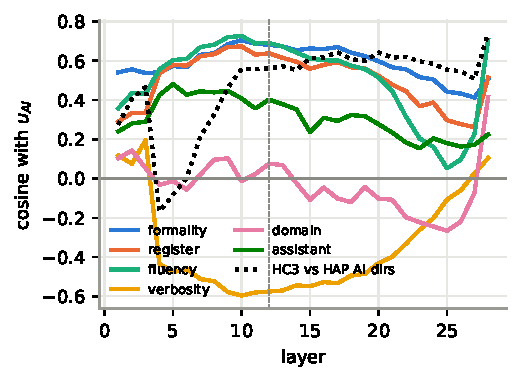
\includegraphics[width=\linewidth]{figures/readout_cosines.pdf}
\end{minipage}\hfill
\begin{minipage}{0.5\linewidth}
\caption{Cosine between $u_{AI}$ and the confound directions across layers (instruct). The dashed vertical line marks the steering layer (12). Each confound direction holds authorship fixed. The dotted line is the agreement between the AI directions fit on HC3 and on HAP. For reference, two random directions in $\mathbb{R}^{3584}$ have $|\cos|\approx 0.02$, and the domain direction stays near 0.}
\label{fig:cosines}
\end{minipage}
\end{figure}

\paragraph{Geometry.} At layer 12, $u_{AI}$ has cosine $0.68$ with formality, $0.69$ with fluency (low NLL), $0.64$ with register, $-0.58$ with verbosity and $0.40$ with the Assistant axis. Its cosine with Reddit-vs-encyclopedic domain is near zero (0.08) (Figure~\ref{fig:cosines}). Projecting $u_{AI}$ onto the 6-dimensional confound span captures 54\% of its squared norm at L12 and 25\% at L27. So the raw direction is roughly half ``formal, fluent, non-verbose, assistant-like'' text. It is clearly \emph{not} the Assistant axis, which it overlaps only moderately and less at late layers ($0.17$ at L27).

\paragraph{The signal is not in the confounds.} Removing the whole confound span and refitting \emph{raises} held-out AUROC at L12, from 0.88--0.91 to 0.97--0.99 on matched sets and from 0.85 to 0.88 on MAGE GPT-4 (Table~\ref{tab:readout}, ``confounds''). Removing a random 6-dimensional subspace changes nothing. The confound-orthogonal direction $u_{AI}^{\perp}$ alone reads out at 0.97--0.99 on matched sets and 0.93 on MAGE GPT-4, far above any single confound direction ($\leq 0.80$). The confounds were mostly adding variance unrelated to authorship. Removing $u_{AI}$ itself and refitting drops AUROC to 0.34--0.71. Much of the linearly decodable signal is concentrated in this one direction, though not all of it (cf.\ INLP~\citep{ravfogel2020null}).

\paragraph{Perplexity.} Perplexity is the strongest scalar confound. AI text is much more likely under Qwen (mean-NLL AUROC 0.79--0.98 on matched sets), and at L12 the raw $u_{AI}$ projection correlates with NLL ($\rho\approx-0.5$ within class). A logistic model on [NLL, length] does not improve when the raw $u_{AI}$ projection at L12 is added (Table~\ref{tab:scalar}; e.g.\ HC3 0.89$\rightarrow$0.90). At this layer the raw direction's read-out is therefore largely a perplexity read-out. The confound-orthogonal $u_{AI}^{\perp}$ behaves differently. It adds substantial information beyond NLL and length (HC3 0.89$\rightarrow$0.98, MAGE GPT-4 0.80$\rightarrow$0.95, content-matched paraphrases 0.68$\rightarrow$0.89), and it keeps AUROC 0.69--0.85 on chat-model text even after NLL and length are regressed out of the projection. Low perplexity is part of what makes text ``sound like AI'', but it is not the whole of what the representation encodes.

\begin{table}[t]
\centering\small
\caption{Scalar confounds at L12 (instruct). AUROC of a logistic model on [mean NLL, log length], with and without the projection on the direction, fit on one half of each eval set and tested on the other. ``Resid.'' is the AUROC of the projection after linearly regressing out NLL and length.}
\label{tab:scalar}
\begin{tabular}{lcccccc}
\toprule
& \multicolumn{3}{c}{$u_{AI}$} & \multicolumn{3}{c}{$u_{AI}^{\perp}$}\\
\cmidrule(lr){2-4}\cmidrule(lr){5-7}
Eval set & NLL+len & +proj & resid. & NLL+len & +proj & resid.\\
\midrule
\tabinput{tables/scalar.tex}
\bottomrule
\end{tabular}
\end{table}

\subsection{Causal test: subtracting the direction makes the model's own answers read as human}
\label{sec:steer}

\begin{table}[t]
\centering\small
\caption{Steering Qwen2.5-7B-Instruct at layer 12, on 160 held-out HC3 questions. Detector and judge columns are means over \emph{English} outputs (\% non-English is the share removed; see text). ``@50w'' = detectors on the first 50 words only, dropping shorter answers (length control). Bino = Binoculars $-B$ (higher = more AI). logit = mean desklib logit, which stays informative where probabilities saturate. Coh./Rel. = Gemma-3 judge, 1--10. Sim = embedding cosine to the unsteered answer to the same question. All control vectors have the same norm as $u_{AI}$ at the same $\alpha$.}
\label{tab:steer}
\setlength{\tabcolsep}{2.6pt}
\begin{tabular}{lrcccccccccr}
\toprule
& \%non- & \multicolumn{2}{c}{P(AI)} & \multicolumn{2}{c}{P(AI) @50w} & & desklib & & & & \\
\cmidrule(lr){3-4}\cmidrule(lr){5-6}
Condition & Engl. & desklib & fakespot & desklib & fakespot & Bino & logit & Coh. & Rel. & Sim & words\\
\midrule
\tabinput{tables/steering.tex}
\bottomrule
\end{tabular}
\end{table}

\begin{figure}[t]
\centering
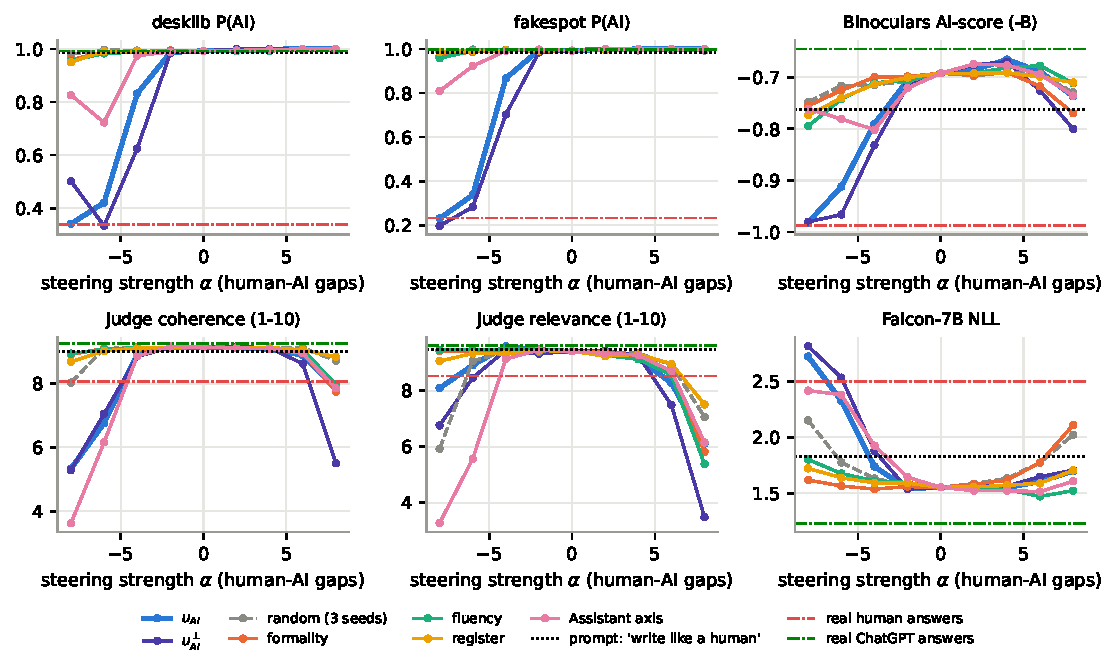
\includegraphics[width=\linewidth]{figures/steering_dose.pdf}
\caption{Dose-response of steering at layer 12, with English outputs only. Negative $\alpha$ pushes towards ``human''. Horizontal lines are the unsteered model's prompt baseline and the real human and ChatGPT answers to the same questions. All directions have equal norm at each $\alpha$.}
\label{fig:dose}
\end{figure}

\begin{table}[t]
\centering\small
\caption{Validation of the independent measures on held-out \emph{real} text: AUROC for separating AI from human text (250 HC3 question pairs; 150 HAP prefixes per generator). The supervised detectors and Binoculars are valid. The Gemma-3 judge's AI-likeness rating is not.}
\label{tab:validation}
\begin{tabular}{lccccc}
\toprule
Contrast & desklib & fakespot & Binoculars & HC3-RoBERTa & judge AI-likeness\\
\midrule
\tabinput{tables/validation.tex}
\bottomrule
\end{tabular}
\end{table}

\paragraph{Validity of the measures.} Before steering we checked every measure on held-out real text (Table~\ref{tab:validation}). Both supervised detectors and Binoculars separate human from AI text almost perfectly (AUROC 0.90--1.00), including base-model text. The Gemma-3-12B judge's AI-likeness rating is near chance (0.46--0.60). It also rates degenerate text as maximally AI-like (Table~\ref{tab:steer_full} in the appendix). We therefore do \textbf{not} use the judge for AI-ness. We keep it only for coherence and relevance, for which it behaves sensibly (unsteered 9.1/9.4; real human answers 8.1/8.5; broken text 1.0). This agrees with the warning in the task framing that LLM judges are noisy on ``sounds like AI''.

\paragraph{Steering towards ``human'' works, and controls do not.} Table~\ref{tab:steer} and Figure~\ref{fig:dose} summarise the results. The unsteered model is detected as AI on essentially every answer (desklib 0.99, fakespot 0.99). Subtracting $u_{AI}$ lowers both supervised detectors and Binoculars, monotonically in $|\alpha|$. At $\alpha{=}{-}6$, mean P(AI) is 0.42 (desklib) and 0.34 (fakespot), and Binoculars moves most of the way from the model ($-0.69$) to real human answers ($-0.99$). The real human answers to the same questions score 0.34/0.23/$-0.99$. Three random directions of identical norm leave the detectors at 0.98--1.00 at every $\alpha$ (paired Wilcoxon $p<10^{-16}$ vs.\ $u_{AI}$ for every detector at $\alpha\leq{-}4$). So did the formality, register and fluency directions (desklib 0.95--0.96 at $\alpha{=}{-}8$) and the Assistant axis (0.72--0.83), even though each of them shares 0.4--0.7 cosine with $u_{AI}$.
\textbf{Length is not the explanation.} Steered answers are shorter, but on only the first 50 words the effect remains (desklib/fakespot 0.69/0.59 at $\alpha{=}{-}6$ and 0.47/0.29 at $\alpha{=}{-}8$, against 0.97/0.95 unsteered and 0.49/0.30 for real human answers).
\textbf{Positive steering} is at the probability ceiling. In logit space it still pushes beyond the unsteered model (desklib logit 8.8 $\rightarrow$ 11.7 at $\alpha{=}{+}8$; random 9.8, formality 9.9). It nearly triples the rate of stock assistant phrases (1.3 $\rightarrow$ 3.4 per 100 words), producing text such as ``\emph{Navigating the landscape of financial challenges can be complex\ldots}''.

\paragraph{Coherence cost and matched-quality comparison.} The effect costs some quality. At $\alpha{=}{-}4$ judge coherence falls only from 9.1 to 8.9, and relevance even rises (9.6), but the detectors only reach 0.83/0.87. At $\alpha{=}{-}6$ coherence is 6.8 (real human answers: 8.1). Two observations show the detector shift is not a by-product of degradation. First, equal-norm random directions at $\alpha{=}{-}8$ degrade coherence comparably (7.6--8.7) without moving the detectors. Second, Table~\ref{tab:matched} keeps only answers the judge rates $\geq 8$ on \emph{both} coherence and relevance. Among these high-quality answers, $u_{AI}$ at $\alpha{=}{-}6$ still scores 0.53/0.42 and $u_{AI}^{\perp}$ scores 0.40/0.30, which matches real human answers that pass the same filter (0.36/0.26). Random and confound directions stay at 0.96--1.00. Figure~\ref{fig:tradeoff} shows the whole frontier: at every coherence level, $u_{AI}$ and $u_{AI}^{\perp}$ dominate all controls.

\paragraph{The confound-orthogonal component is the better steering vector.} $u_{AI}^{\perp}$ has no component along formality, register, fluency, verbosity, domain or the Assistant axis. It steers \emph{at least as well} as $u_{AI}$ (desklib 0.62 vs.\ 0.83 at $\alpha{=}{-}4$, at equal coherence 8.8--8.9; 0.33 vs.\ 0.42 at $\alpha{=}{-}6$), and it almost never switches language (1\% vs.\ 13\% at $\alpha{=}{-}6$). The causal effect on detectors therefore does not run through the measured confounds.

\paragraph{The prompt baseline barely moves the detectors.} Asking the model to answer ``like an ordinary person on Reddit, not like an AI'' changes the surface: ``Hey there!'', fewer lists, more contractions. But detectors still flag 99\% of answers (desklib 0.99, fakespot 0.98, Binoculars $-0.76$). Prompt plus steering ($\alpha{=}{-}4$) reaches 0.68/0.60 at coherence 7.8, slightly better than steering alone at that coherence. The direction captures something the model does not change when merely instructed to sound human.

\paragraph{What changes in the text.} Under negative steering, answers lose markdown lists and stock assistant phrases (``it is important to'', ``generally'', ``consult''; 1.3 $\rightarrow$ 0.4 per 100 words at $\alpha{=}{-}6$). They also get shorter, more direct and more first-person (Figure~\ref{fig:style} and Table~\ref{tab:examples} in the appendix). Content is largely preserved at moderate strength. The embedding similarity to the unsteered answer is 0.84 at $\alpha{=}{-}4$ and 0.78 at $\alpha{=}{-}6$, against 0.91 between two unsteered samples with different seeds and 0.67 between the model's answer and the real human answer.

\paragraph{Failure modes.} (i)~\emph{Language switching}: strong negative steering with $u_{AI}$ sometimes makes the model answer in Chinese (3\% at $\alpha{=}{-}4$, 13\% at $-6$, 38\% at $-8$). The fluency direction does this too (22\% at $-8$). English-trained detectors are not valid on such text, so all reported numbers exclude these outputs. With them included, the detector scores are similar or lower (Appendix~\ref{app:full}). That $u_{AI}^{\perp}$ rarely switches language suggests the switching runs through the fluency/low-NLL component: for Qwen, much of its most ``fluent'' mass may be Chinese.
(ii)~\emph{Multi-layer interventions are brittle}. Adding $\alpha g_\ell u_{AI,\ell}$ at all 27 layers works at $\alpha{=}{-}0.25$ (desklib 0.71 at coherence 7.2). At $|\alpha|\geq 0.5$ it destroys coherence. Clamping every token's projection to the human mean at all layers (a directional ablation) produces gibberish (coherence 1.1). The direction is defined by \emph{mean-pooled} statistics, and forcing every token to the pooled mean is far outside the data distribution.

\begin{table}[t]
\centering\small
\caption{Matched-quality comparison: mean detector P(AI) over English answers that the judge rates $\geq8$ for \emph{both} coherence and relevance, and the share of answers that pass the filter.}
\label{tab:matched}
\setlength{\tabcolsep}{3.2pt}
\begin{tabular}{lccccccccc}
\toprule
& \multicolumn{3}{c}{$\alpha{=}{-}4$} & \multicolumn{3}{c}{$\alpha{=}{-}6$} & \multicolumn{3}{c}{$\alpha{=}{-}8$}\\
\cmidrule(lr){2-4}\cmidrule(lr){5-7}\cmidrule(lr){8-10}
Direction & desklib & fakespot & kept & desklib & fakespot & kept & desklib & fakespot & kept\\
\midrule
\tabinput{tables/matched_quality.tex}
\bottomrule
\end{tabular}
\end{table}

\begin{figure}[t]
\centering
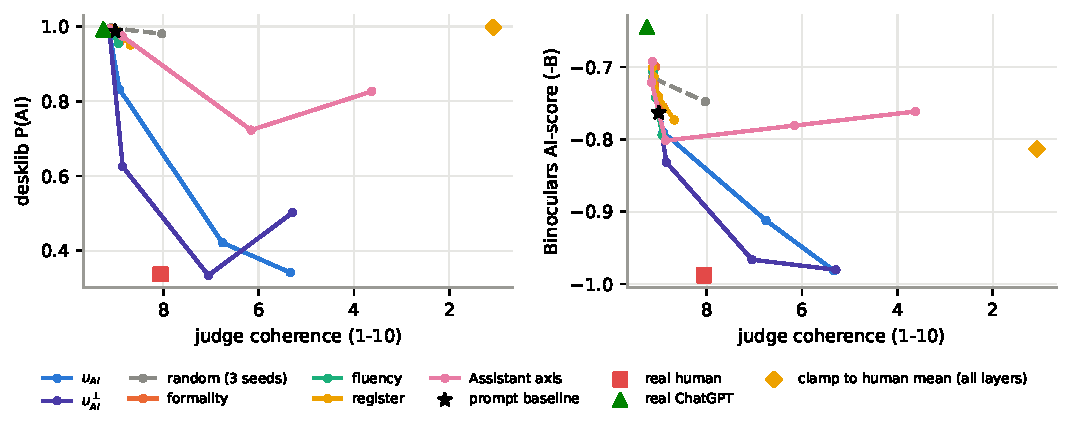
\includegraphics[width=\linewidth]{figures/steering_tradeoff.pdf}
\caption{Detector score vs.\ judge coherence for each steering family as $|\alpha|$ grows (negative $\alpha$; the curves start at the unsteered model, top left). Lower and further left is better. Markers show the prompt baseline, real human and ChatGPT answers, and all-layer clamping.}
\label{fig:tradeoff}
\end{figure}

\subsection{Base vs.\ instruct: the direction predates chat tuning}
\label{sec:base}

\begin{figure}[t]
\centering
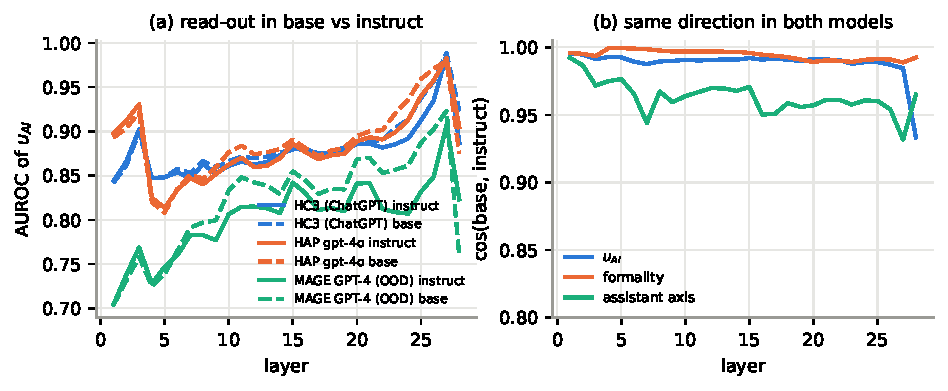
\includegraphics[width=\linewidth]{figures/base_vs_instruct.pdf}
\caption{(a) Read-out AUROC of $u_{AI}$ fit separately in the base (dashed) and instruct (solid) model. (b) Cosine between the base and instruct versions of $u_{AI}$, the formality direction and the Assistant axis, at each layer.}
\label{fig:base}
\end{figure}

We repeated the read-out in the pretrained Qwen2.5-7B, fitting all directions afresh from its own activations. The AI direction in the base model is nearly identical to the instruct one: cosine 0.98--0.995 at every layer from 1 to 27 (Figure~\ref{fig:base}b). Its read-out AUROC is equal or slightly higher, by 0.005--0.018 on average across layers. The base direction applied to instruct activations reads out as well as the instruct direction (0.87 vs.\ 0.86 on HC3 at L12). Chat tuning therefore neither created nor measurably amplified the representation \emph{of} AI-sounding text. The Assistant axis is also largely shared (cosine $\geq0.93$), as \citet{lu2026assistant} report. One caveat: Qwen2.5's pretraining data postdates ChatGPT and likely contains AI-written text, so ``base'' does not mean ``never saw AI text''.

The base direction is also causal in the base model (Table~\ref{tab:base}). We continue 160 held-out human text prefixes from HAP. Desklib already flags unsteered Qwen base continuations as AI (0.97). Subtracting $u_{AI}^{base}$ lowers this to 0.63 ($\alpha{=}{-}4$) and 0.43 ($\alpha{=}{-}8$), while an equal-norm random direction does not (0.96/0.94). Adding it makes continuations of human fiction and news sound like an assistant: the stock-phrase rate rises ninefold (0.22 $\rightarrow$ 1.99 per 100 words) and the desklib logit rises from 5.7 to 11.7 (random: 7.6). One example continues a Victorian children's story with ``\emph{Together, they spent countless hours exploring the world\ldots\ Despite the challenges that life presented, the child grew stronger and more resilient}''. So the pretrained model already has a steerable ``assistant voice'', which chat tuning then makes the default.

\begin{table}[t]
\centering\small
\caption{Steering the \emph{base} model (Qwen2.5-7B) with its own $u_{AI}$ at L12, continuing 160 human text prefixes. AI-phr = stock assistant phrases per 100 words. Coh. = judge coherence.}
\label{tab:base}
\begin{tabular}{lccccccc}
\toprule
Condition & desklib & fakespot & Bino & desklib logit & AI-phr & Coh. & words\\
\midrule
\tabinput{tables/base_steering.tex}
\bottomrule
\end{tabular}
\end{table}

\section{Discussion}
\label{sec:discussion}

\paragraph{Is there a ``sounds like AI'' direction?} In the sense we can test, yes. A single direction, read off from \emph{other} models' text, has three properties. (a)~It separates human from chat-model text across corpora, generators and content-matched paraphrases. (b)~Subtracting it makes Qwen's own answers read as human-written to detectors that never saw Qwen's activations, at the level of real human answers once quality is held fixed. (c)~Adding it makes both the chat model and the \emph{base} model write in recognisable assistant prose. Equal-norm random directions do none of this, and neither do the four confound directions or the Assistant axis.

\paragraph{What it is and is not.} It is not ``machine-generated'' in general: base-model and pre-chat text is invisible to it. It is also not the Assistant persona. Its cosine with the Assistant axis is moderate (0.40 at L12, 0.17 at L27), and steering with the Assistant axis mostly breaks coherence and relevance rather than humanising the text (Table~\ref{tab:steer}). About half of the raw direction is formality, fluency, register and terseness, which is unsurprising since those are real differences between chat-model and human text. But the part orthogonal to all measured confounds both reads out \emph{better} and steers \emph{better}. The most natural description is a learned representation of \emph{chat-assistant register}: the house style that post-trained models share across vendors. Pretraining corpora that contain such text already teach the base model this representation, and chat tuning moves the model's default output to its far end without changing the axis itself.

\paragraph{Implications for detection.} Prompting the model to ``sound human'' left 99\% of answers detectable. A single-vector intervention at one layer brought detection close to the level of real human text at matched quality, at a cost of a few dozen lines of code. This is a form of detector evasion. We report it because the result bears directly on how much detectors can be trusted: current detectors (and, plausibly, activation probes) key on a low-dimensional feature that the generating model itself represents and can turn down. Detectors should be stress-tested against such activation-level attacks in addition to paraphrasing~\citep{krishna2023paraphrasing,sadasivan2023can}. Conversely, the direction gives a cheap, model-internal handle for \emph{auditing} how much a model's output relies on assistant register.

\section{Limitations}
\label{sec:limitations}

\begin{itemize}
    \item \textbf{One model family.} All causal results are on Qwen2.5-7B (base and instruct) at one steering layer. We did not test Gemma or Llama models, SAE-feature-level analyses~\citep{kuznetsov2025feature}, or larger models.
    \item \textbf{Detectors are proxies.} ``Reads as human'' means ``scored as human by two supervised detectors and Binoculars''. We did not run a human study. The Gemma-3 judge could not tell human from AI text on our validation set (AUROC $\leq$0.60), so the claim rests on the detectors. We also cannot rule out that all three detectors share blind spots that the direction exploits.
    \item \textbf{Quality cost.} The strongest effects ($\alpha{\leq}{-}6$) cost coherence (judge 6.8--7.1 vs.\ 8.1 for real human answers) and sometimes switch the output language. At near-zero coherence cost ($\alpha{=}{-}4$) the effect is partial (P(AI) 0.62--0.87). Our coherence and relevance scores come from a single LLM judge.
    \item \textbf{Confound set is finite.} We controlled six named confounds with authorship held fixed. Other correlates of chat style (e.g.\ hedging, markdown habits, specific lexical items) are not separated out and may be part of $u_{AI}^{\perp}$. Some confound directions are themselves AI-generated (formality rewrites by Llama-3.1).
    \item \textbf{Base model is not pre-AI.} Qwen2.5 was pretrained after ChatGPT, so its base model has likely seen assistant-style text. Our base-vs-instruct result says chat tuning did not \emph{create} the direction in this model. It does not say that the direction would exist in a model trained only on pre-2022 data.
    \item \textbf{Datasets.} We used HC3, the human-AI parallel corpus and MAGE. We did not use RAID: its public test split is unlabelled and the labelled training split is 12\,GB. Some HC3 human answers are low-quality Reddit posts, which is part of why human answers score lower on coherence.
\end{itemize}

\section{Conclusion}
\label{sec:conclusion}

The residual stream of Qwen2.5-7B contains a direction for ``sounds like an AI assistant''. It is fit from other models' text, it transfers across generators and corpora, and it is causal for the model's own writing: removing it makes outputs read as human to independent detectors far better than prompting does, and adding it produces stock assistant prose even in the base model. It is not the Assistant persona and not just formality or fluency. Its confound-orthogonal component is the cleanest version for both reading and writing. The direction already exists before chat tuning. Chat tuning appears to change where the model sits along it, not the axis itself.

\paragraph{Reproducibility.} All code, raw outputs and analysis scripts are in the accompanying repository (\texttt{src/}, \texttt{results/}). Every number in this paper is produced by those scripts.


\bibliographystyle{plainnat}
\bibliography{references}

\appendix
\section{Layer pilot}
\label{app:pilot}

\begin{table}[h]
\centering\small
\caption{Layer$\times$strength pilot (instruct model, $u_{AI}$, 40 prompts, all outputs including non-English). Falcon NLL is a fluency proxy (real human answers: 2.50). Sim = embedding cosine to the unsteered answer. Layer 12 gave the largest detector change at moderate fluency cost. At layers 20--24, strong steering in either direction produces degenerate text (very low Sim), which fakespot scores as human but desklib does not.}
\label{tab:pilot}
\setlength{\tabcolsep}{4pt}
\begin{tabular}{rrrcccccr}
\toprule
Layer & $\alpha$ & \%non-Engl. & desklib & fakespot & Bino & Falcon NLL & Sim & words\\
\midrule
\tabinput{tables/pilot.tex}
\bottomrule
\end{tabular}
\end{table}

\section{Full steering results}
\label{app:full}

\begin{table}[h]
\centering\scriptsize
\caption{All main-grid conditions (layer 12 unless stated; ``addall'' = all layers). ``All'' columns include non-English outputs; ``EN'' columns are English only. The judge's AI-likeness is shown for completeness. It is not a valid measure (Table~\ref{tab:validation}): it gives degenerate outputs (clamp, addall $\pm1$) the maximum score.}
\label{tab:steer_full}
\setlength{\tabcolsep}{3pt}
\begin{tabular}{lrcccccccccc}
\toprule
& & \multicolumn{3}{c}{all outputs} & \multicolumn{2}{c}{EN} & \multicolumn{3}{c}{judge (EN)} & \\
\cmidrule(lr){3-5}\cmidrule(lr){6-7}\cmidrule(lr){8-10}
Condition & \%non-EN & desklib & fakespot & Bino & desklib & fakespot & AI-like & Coh. & Rel. & Falcon NLL\\
\midrule
\tabinput{tables/steer_full.tex}
\bottomrule
\end{tabular}
\end{table}

\begin{figure}[h]
\centering
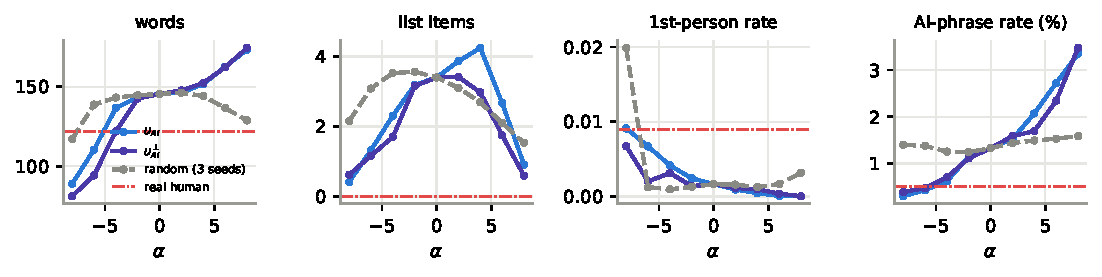
\includegraphics[width=\linewidth]{figures/steering_style.pdf}
\caption{Stylometrics under steering at layer 12 (English outputs). The AI-phrase rate counts a fixed list of stock assistant phrases (``it is important to'', ``overall,'', ``additionally'', ``consult'', ``various'', \dots) per 100 words.}
\label{fig:style}
\end{figure}

\section{Examples}
\label{app:examples}

\begin{table}[h]
\centering\scriptsize
\caption{Excerpts of outputs (first $\sim$45 words, verbatim) for two held-out prompts. Same seed across conditions.}
\label{tab:examples}
\begin{tabular}{p{0.17\linewidth}p{0.78\linewidth}}
\toprule
\multicolumn{2}{l}{\emph{Prompt (HC3 open\_qa): ``what is Polyester in packaging PET''}}\\
\midrule
unsteered & PET stands for Polyethylene Terephthalate, which is a type of polyester used extensively in the manufacturing of packaging materials. Here's an overview: \#\#\# Properties of PET: - **Strength and Durability**: PET is strong and durable, making it suitable for various packaging applications.\\
prompt ``like a human'' & Hey there! When you hear about polyester in packaging PET, it's basically talking about using polyester materials in the production of PET (polyethylene terephthalate) containers or films. PET is a type of plastic widely used for bottles and packaging because it's lightweight, shatter-resistant, and recyclable.\\
$u_{AI}$, $\alpha{=}{-}6$ & Polyester (PET) is a polymer compound, and it's widely used in the production of bottles, fibers and others. PET has good mechanical property, transparency, and economical price, so it's wide used in food packging.\\
$u_{AI}^{\perp}$, $\alpha{=}{-}4$ & Polyester (PET or PETE) is a thermoplastic polymer resin of the polyester family of polymers. It is used in fibres for clothing, bottles, plastic films for food wrapping and general use, and synthetic fibers for textiles among others. PETG is a copolymer modification which improves some processing behaviour.\\
random, $\alpha{=}{-}6$ & Polyester, often referred to in the context of packaging materials like PET (Polyethylene Terephthalate), is a type of plastic commonly used for bottles, containers, and wraps. [\dots] Here's what you need to know about PET in packaging: 1. **Material Composition**: \dots\\
$u_{AI}$, $\alpha{=}{+}8$ & Polyester is a type of material commonly used in various applications, particularly in the food industry. It is made from synthetic polymers that can be molded into different shapes and forms to create packaging for products such as beverages, medications, and other goods.\\
\midrule
\multicolumn{2}{l}{\emph{Prompt (HC3 ELI5): ``Communism. If this has been asked before, I apologize. Explain like I'm five.''}}\\
\midrule
unsteered & Sure! Imagine you have a big cookie jar, and there are lots of cookies inside. Communism is like saying everyone should share the cookies equally, so no one person gets too many and others don't get any.\\
$u_{AI}$, $\alpha{=}{-}4$ & [answers in Chinese: an informal, opinionated explanation; example of language switching]\\
$u_{AI}^{\perp}$, $\alpha{=}{-}4$ & OK, let's try this: Imagine the whole world is a big pie. Now imagine that all the people who live in this world, are actually equal and none is superior to others. Now comes the difficult part: how to share the pieces of the pie.\\
$u_{AI}$ all layers, $\alpha{=}{+}0.5$ & Imagine a world where everyone works together to create a community that priorit, fairness, and equality. Imagine a society where individuals come together to support one another, fostering a sense of unity and shared goals.\\
\midrule
\multicolumn{2}{l}{\emph{Base model, continuing a 19th-century children's story (``\dots She had one companion, a boy-cousin about a year older than herself.'')}}\\
\midrule
unsteered & He was a wild, mischievous, and in some respects a very disagreeable little creature; but she was so accustomed to his society that she seemed to enjoy it more than that of any other child.\\
$u_{AI}^{base}$, $\alpha{=}{-}8$ & But that boy was a regular scamp of a kid, and she was a regular spoiled kid. That boy was bad boy. Both were orphans.\\
$u_{AI}^{base}$, $\alpha{=}{+}8$ & Together, they spent countless hours exploring the world, and learning the intricacies of the human mind. They reveled in the joys of discovery, and the thrill of new experiences, and the sense of adventure that came with each passing moment.\\
\bottomrule
\end{tabular}
\end{table}

\section{Additional details}
\label{app:details}

\paragraph{Assistant-axis personas.} Pirate captain, medieval peasant farmer, grumpy fisherman, teenage skateboarder, Shakespearean actor, 1940s detective, cowboy, forest spirit, Viking warrior, sarcastic comedian, nervous medical student, Victorian aristocrat, surfer, Roman senator, conspiracy theorist, kindergarten teacher, drill sergeant, romantic poet, Mumbai street vendor, night-shift nurse, hip-hop artist, fantasy wizard, talking dog, ghost. Each persona was given the system prompt ``You are [persona]. Stay fully in character at all times; never mention being an AI or an assistant.'' and answered 16 everyday questions (160 tokens, $T{=}0.7$).

\paragraph{Judge prompt.} The judge sees the question and the response (truncated to 300 words) and is asked for a JSON object with integer 1--10 ratings of \texttt{ai\_likeness}, \texttt{coherence} and \texttt{relevance}, defined as in \S\ref{sec:method}. Base-model continuations are framed as ``(Continue the following passage) \dots'' followed by the last 60 words of the prefix.

\paragraph{Compute.} One NVIDIA RTX A6000 (48\,GB). Activation extraction for both models took $\sim$25 minutes. The main steering grid (87 conditions $\times$ 160 prompts) took $\sim$50 minutes. Detector scoring took $\sim$35 minutes and judging with vLLM $\sim$20 minutes.

\end{document}
